\documentclass{article}

\usepackage{tikz}

\begin{document}

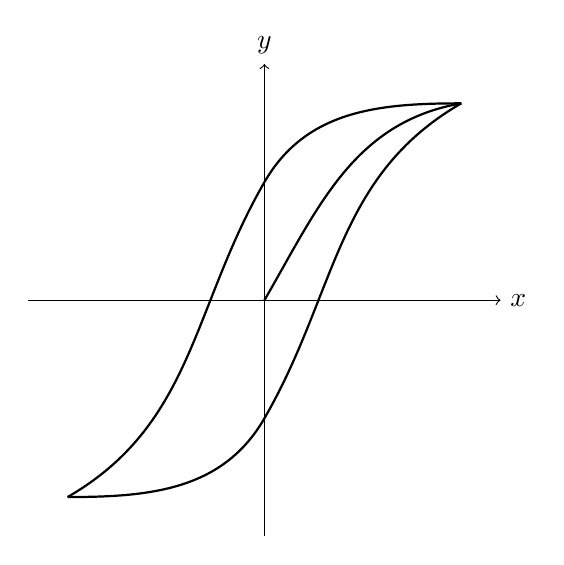
\begin{tikzpicture}
  [hysteresis/.style = {thick}]

% Axes
\draw[->] (-3,0) -- (3,0) node[right] {$x$};
\draw[->] (0,-3) -- (0,3) node[above] {$y$};

% First curve
\draw[hysteresis] (0,0) to [out=60,in=190] (2.5,2.5);

% Second curve
\draw[hysteresis] (2.5,2.5) to [out=180,in=60] (0,1.5);
\draw[hysteresis] (0,1.5) to [out=240,in=30] (-2.5,-2.5);

% Third curve
\draw[hysteresis] (-2.5,-2.5) to [out=0,in=240] (0,-1.5);
\draw[hysteresis] (0,-1.5) to [out=60,in=210] (2.5,2.5);

\end{tikzpicture}

\end{document}
